\chapter{Location and Thickness of Boundary Layers}
\paragraph{Example 1:} Consider
\begin{gather*}
	\epsilon y'' - y' + y = 0 \\
	y(0) = 0 \qquad y(1) = 1
\end{gather*}
First we find the \underline{outer solution}, i.e. $\epsilon \rightarrow 0^+$:
\begin{gather*}
	-y_0' + y_0 = 0 \qquad \implies y_0 = A \me^x
\end{gather*}
But which BC to apply? In BL we expect the solution to decay exponentially as we move away from the BL. Since the solution is growing, we expect the BL to be at the right boundary such that as we move into the domain, the solution decays. So we expect the BL to be at $x=1$. \\
\ \newline 
But let's suppose the BL is at $x=0$. Then we apply the BC at $x=1$, i.e.
\begin{gather*}
	y_0(x)_\text{out} = \me^{x-1}
\end{gather*}
The \underline{inner solution}: Still assuming the BL at $x=0$, we assume thickness $O(\delta)$, where $\delta = \delta(\epsilon)$ is to be determined. Let 
\begin{gather*}
	X = \frac{x}{\delta}
\end{gather*}
and we are interested in the ODE
\begin{gather*}
	y(x)_\text{inn} = Y(X)
\end{gather*}
which is achieved through
\begin{align*}
	y' &= \frac{\md y}{\md x} = \frac{\md Y}{\md X} \frac{\md X}{\md x} = \frac{1}{\delta} Y_X \\
	y'' &= \frac{\md y'}{\md X} \frac{\md X}{\md x} = \frac{1}{\delta^2} Y_{XX}
\end{align*}
Note that since the ODE is linear, we can always write $Y = c y$ without affecting the equation. But in nonlinear (and some linear) problems, this $c$ is to be determined. Our ODE becomes
\begin{gather*}
	\epsilon \frac{1}{\delta^2} Y_{XX} - \frac{1}{\delta} Y_X + Y = 0
\end{gather*}
We now make a \underline{dominant balance} argument: if we have chosen $\delta$ correctly, it would mean that $Y,Y_X,Y_{XX}$ are $O(1)$. Is it then
\begin{enumerate}
	\item As $\epsilon \rightarrow 0^+$ \begin{gather*}
		\frac{\epsilon}{\delta^2} \approx \frac{1}{\delta} \gg 1 ?
	\end{gather*}
	This would mean $\delta \approx \epsilon $ and $\ll 1$ which is consistent. 
	\item It is also possible that
	\begin{gather*}
		\frac{\epsilon}{\delta^2} \approx 1 \gg \frac{1}{\delta}
	\end{gather*}
	Therefore $\delta \approx \epsilon^{1/2} \ll 1$. But the ordering suggests $\delta \gg 1$, i.e. inconsistent.
	\item Finally, 
	\begin{gather*}
		\frac{1}{\delta} \approx 1 \gg \frac{\epsilon}{\delta^2}
	\end{gather*}  
	This means $\delta \approx 1$ and $\epsilon \ll 1$. The latter is OK, but $\delta \approx 1$ means the outer solution and not the inner, i.e. layer, solution!  
\end{enumerate}
So we conclude that the BL has a thickness
\begin{gather*}
	\delta = O(\epsilon) \quad \implies \delta = \epsilon
\end{gather*}
and if only \emph{one case} gives a consistent and non-trivial balance (i.e. not the outer solution), we refer to it as a ``distinguised limit''. 
\begin{itemize}
	\item Whilst this analysis is predicated on the wrong assumption about the location of the BL, nevertheless, the argument to determine the thickness is correct.
	\item We know the position of the BL is incorrect as we will fail to match the inner and outer solutions. 
\end{itemize}
Our ODE for the inner problem is finally
\begin{gather*}
	Y'' - Y' + \epsilon Y = 0 \\
	Y(0) = 0
\end{gather*}
Proceeding with the usual ansatz we derive
\begin{gather*}
	(Y_0'' + \epsilon Y_1'' + \dots) - (Y_0' + \epsilon Y_1' + \dots ) + \epsilon (Y_0 + \epsilon Y_1 + \dots) = 0
\end{gather*}
This yields at $O(\epsilon^0)$
\begin{gather*}
	Y_0'' - Y_0' = 0
\end{gather*}
Solving this
\begin{gather*}
	Y_0(X) = B(1 - \me^{X})
\end{gather*}
Our solution is growing exponentially away from $x = 0$ -- this is a sign of trouble! Solutions usually decay away from the end-point of the BL. Let's try to match:
\begin{align*}
	\lim\limits_{X \rightarrow \infty} Y_0(X)_\text{inn} &= \lim\limits_{x \rightarrow 0} y_0(x)_\text{out} \\
	-B(\infty)&= \me^{-1}
\end{align*}
The matching is impossible and this is because we incorrectly guessed the location of the BL. If instead we took the BL at $x=1$
\begin{gather*}
	y_0(x)_\text{out} = A\me^x
\end{gather*}
and the BC of interest is that at $x=0$, i.e. $A=0$ and
\begin{gather*}
	y(x)_\text{out} = 0
\end{gather*}
to all orders as can be easily checked. Now we are used to $X \rightarrow \infty$ in our BL when the BL is near $x=0$. \\
\ \newline 
If the BL is at $x=1$, we take
\begin{gather*}
	X = \frac{1-x}{\delta} \\
	0 \leq x \leq 1 \qquad 0 \leq X \leq \frac{1}{\delta}
\end{gather*}
Proceeding like previously
\begin{align*}
y' &= \frac{\md y}{\md x} = \frac{\md Y}{\md X} \frac{\md X}{\md x} = -\frac{1}{\delta} Y_X \\
y'' &= \frac{\md y'}{\md X} \frac{\md X}{\md x} = \frac{1}{\delta^2} Y_{XX}
\end{align*}
and our ODE becomes
\begin{gather*}
	Y_{XX} + Y_X + \epsilon Y = 0
\end{gather*}
Notice the positive sign on $Y_X$ with was negative previously. Solving this at $O(\epsilon^0)$
\begin{gather*}
	Y_0(x) = C + D\me^{-X} \\
	Y_0(0) = 1 = C+D
\end{gather*}
since we are looking at $x=1$ or $X=0$. Therefore
\begin{gather*}
	Y_0(X) = C + (1-C)\me^{-X}
\end{gather*}
and matching this
\begin{align*}
	\lim\limits_{X \rightarrow \infty} Y_0(X) &= \lim\limits_{x \rightarrow 1} y_0(x) \\
	C&= 0
\end{align*}
The composite solution at $O(\epsilon^0)$ is therefore
\begin{align*}
	y_c &= y_\text{out} + Y_\text{inn} - y_\text{match} \\
	&= 0 + \me^{-X} - 0 \\
	&= \me^{(x-1)/\epsilon} + O(\epsilon)
\end{align*}
Note that our matched asymptotic does not satisfy the value at the left boundary. It just so happens to be transcedentally small and gets the BC $\sim$negligibly wrong. 

\paragraph{Useful shortcut:} For general second order BVP of the form
\begin{gather*}
	\epsilon y'' + a(x) y' + b(x) y = 0 \\
	y(0) = A \qquad y(1) = B
\end{gather*}
Note this equation is (1) linear in $y$ and (2) homogeneous. Then
\begin{itemize}
	\item if $a(x)>0$ for all $x \in [0,1]$ then BL is at $x=0$
	\item if $a(x)<0$ for all $x \in [0,1]$ then BL is at $x=1$
	\item if $a(x)=0$ somewhere in $x \in [0,1]$ then we can have an \underline{interior layer}.
\end{itemize}


\paragraph{Example 2:} 
\begin{gather*}
	\epsilon y'' + x^2 y' - y =0 \\
	y(0) = 1 \qquad y(1) = 1
\end{gather*}
Note that $a(x)=0$ at the left end point and not strictly greater than zero. This only means there is a layer at zero. Proceeding as usual, the \underline{outer} solution is found by setting $\epsilon=0$, which yields
\begin{gather*}
	y_0 = A \me^{-1/x}
\end{gather*}
Applying the BC at $x=1$
\begin{gather*}
	y_0(x) = \me^{1-1/x}
\end{gather*}
To solve the \underline{inner} problem, set
\begin{gather*}
	X = \frac{x}{\delta} \\
	X = O(1) \qquad \delta \ll 1
\end{gather*}
which leads to
\begin{gather*}
	\epsilon \frac{1}{\delta^2} Y_{XX} + X^2 \delta^2 \frac{1}{\delta}Y_X - Y = 0
\end{gather*}
Next consider the three balances again. The consistent dominant balance is
\begin{gather*}
	\frac{\epsilon}{\delta^2} \approx 1 \gg \delta \qquad 
	\implies \delta \approx \epsilon^{1/2}
\end{gather*}
Our governing innder ODE is then
\begin{gather*}
	Y'' + \epsilon^{1/2}X^2 Y' - Y = 0
\end{gather*}
with our trial solution reading
\begin{gather*}
	Y = Y_0 + \epsilon^{1/2} Y_1 + \epsilon Y_2 + \dots 
\end{gather*}
At $O(\epsilon^0)$
\begin{gather*}
	Y_0 '' - Y_0 = 0 \qquad Y_0(0) = 1
\end{gather*}
Solving this we arrive at
\begin{gather*}
	Y_0(X) = A \me^{X} + B\me^{-X}
\end{gather*}
Now observe that our matching condition requires taking $X \rightarrow \infty$. Therefore, with this forethought, we set $A=0$. The BC now means that $B=1$. Together
\begin{gather*}
	Y_0(X)_\text{inn} = \me^{-X}
\end{gather*}
Observe that both inner and outer solutions match, with $y_\text{match}=0$, in the overlap region. The composite solution is then
\begin{align*}
	y_c = \me^{1-1/x} + \me^{-x/\sqrt{\epsilon}} + O(\epsilon^{1/2})
\end{align*} 
{\bf NB.} Suppose we wanted to go to the next order, we would need $O(\epsilon)$ terms in $y_\text{out}$, which means we would need one more term in the outer, yet two more terms in the inner: $O(\sqrt{\epsilon})$ and $O(\epsilon)$. The inner solution takes twice the effort!
\begin{figure}[!h]
	\centering
	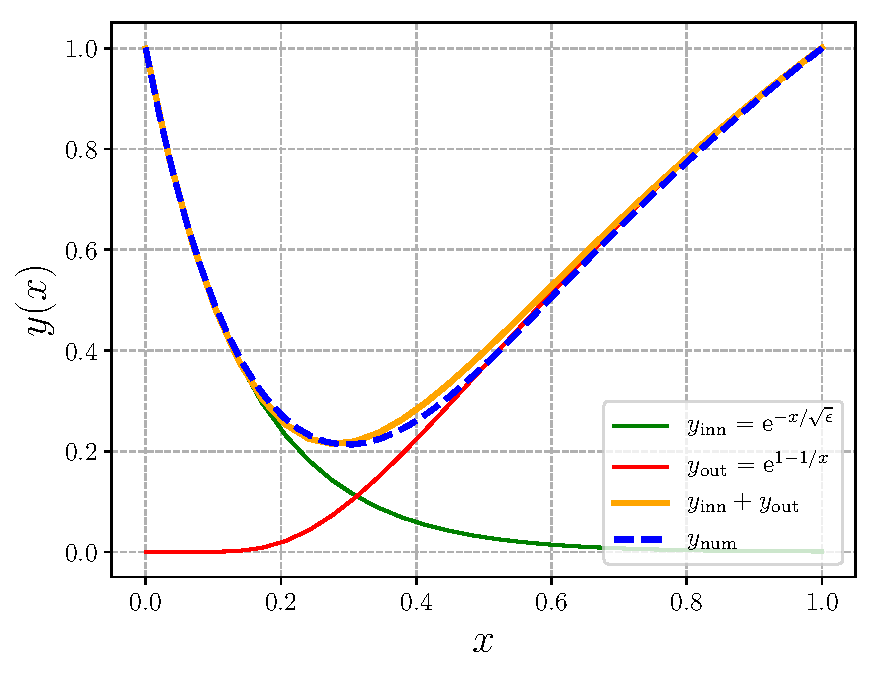
\includegraphics[width=0.65\textwidth]{./plots/pdf/strogatz-wk14.pdf}
	\caption{Various solution terms with $\epsilon=0.02$. Notice the thickness of the boundary layer.}
	\label{fig:strogatz-wk14}
\end{figure} \\








